\documentclass[a4paper,12pt]{extarticle}
\usepackage{geometry}
\usepackage{multirow}
\usepackage{array}
\usepackage{caption} 
\captionsetup[table]{skip=20pt}
\usepackage{imakeidx}
\usepackage{graphicx}
\usepackage[T1]{fontenc}
\usepackage{titling}
\usepackage[utf8]{inputenc}
\usepackage{csquotes}
\usepackage{subcaption}
\usepackage{floatrow} 
\usepackage{float}
\floatstyle{plaintop}
\restylefloat{table}
\usepackage[export]{adjustbox}
\geometry{textwidth=13.9cm}
\renewcommand\maketitlehooka{\null\mbox{}\vfill}
\renewcommand\maketitlehookd{\vfill\null}
\title{{\Huge \textbf{Software Lab 4: \\ \vspace{0.20cm} TeX Lab\vspace{0.5cm}}}}
\author{\LARGE{Diptesh Kanojia \vspace{0.3cm}}}
\date{\Large{21st August, 2019}}
\setlength{\footskip}{50pt}

\usepackage{bera}
%\usepackage{lipsum}

%\usepackage{slantsc}
%\pagestyle{empty}

\begin{document}
  \newdimen\origiwspc%
  \newdimen\origiwstr%
  \origiwspc=\fontdimen2\font% original inter word space
  \origiwstr=\fontdimen3\font% original inter word stretch
\fontdimen3\font=\origiwstr% (original) inter word stretch
  \fontdimen2\font=0.32em% inter word space
 % \lipsum[1]% increased inter word space and stretch
\normalfont
\begin{titlingpage}
\maketitle

\end{titlingpage}
\newpage
\vspace*{0.5cm}
\begin{figure}[h!]
	\centering
	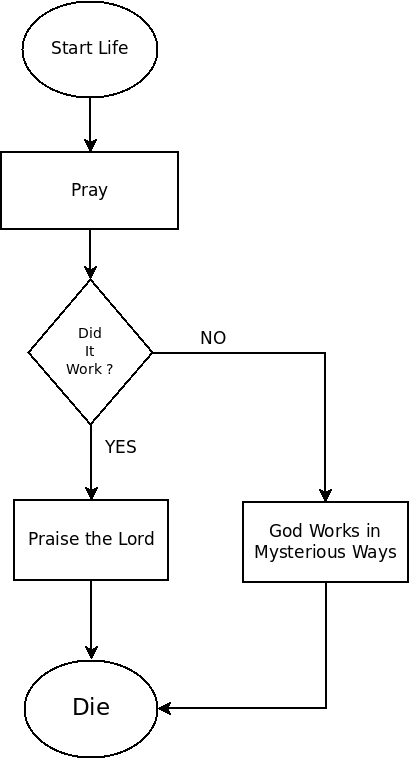
\includegraphics[scale=0.5]{LifePray}
	\vspace{-0.15 cm}
	{\large{\caption{Flowchart of a theist Life}
	\label{fig:lifepray}}}
\end{figure}


Figure \ref{fig:lifepray} above refers to a funny conundrum theists are believed to
be living in by the atheists. This is just a joke I picked up from some
forum, not taking sides, not even a bit. This is how scared social media
has made us, We can not pick sides. Moving on .... You need to know
how to cite papers in \LaTeX. For e.g. you are talking about research
on Indowordnet [1], in that case such a citation must be used near a
name. In case you need to quote the authors of a paper in a statement,
instead of citing them against a topic or word or a line, you need to use
a different kind of citation methodology.

\newpage
\vspace*{0.5cm}
  \begin{table}[h]
  \small\addtolength{\tabcolsep}{-3pt}
\centering
\caption{Table depicting the use of both multirow and multicolumn}

    \begin{tabular}{cc|c|c|c|c|c|c|c|c|c|}
     \cline{3-11}
     & & \multicolumn{5}{c|}{\textbf{Basic Properties}} & \multicolumn{4}{c|}{\textbf{Readability}}\\ \cline{3-11}
\cline{3-11}
   &&\textbf{WC} & \textbf{SC} & \textbf{C-W} & \textbf{S-W} & \textbf{W-S} & \textbf{FK} & \textbf{GF} & \textbf{SMOG} & \textbf{LEX}\\
\cline{1-11}
\multicolumn{1}{|c}{\multirow{2}{*}{Baseline}}&\multicolumn{1}{|c|}{Mean}& 0.84 & 0.41 & \textbf{0.56} & \textbf{0.46} & \textbf{0.65} & \textbf{0.60} & 0.56 & 0.57 & 0.63\\ \cline{2-11}
\multicolumn{1}{|c}{\multirow{2}{*}{}}&\multicolumn{1}{|c|}{SD}& 0.64 & 0.01 & 0.36 & 0.26 & 0.45 & 0.63 & 0.51 & 0.27 & 0.93\\ \hline
\hline
\multicolumn{1}{|c}{\multirow{2}{*}{ScaCom$p_h$}}&\multicolumn{1}{|c|}{Mean}& 0.84 & 0.41 & 0.56 & 0.46 & 0.65 & 0.60 & 0.56 & 0.57 & 0.63\\ \cline{2-11}
\multicolumn{1}{|c}{\multirow{2}{*}{}}&\multicolumn{1}{|c|}{SD}& 0.64 & 0.01 & 0.36 & 0.26 & 0.45 & 0.63 & 0.51 & 0.27 & 0.93\\ \hline
\hline
\multicolumn{1}{|c}{\multirow{2}{*}{ScaCom$p_l$}}&\multicolumn{1}{|c|}{Mean}& \textbf{0.84} & \textbf{0.41} & 0.56 & 0.46 & 0.65 & 0.60 & \textbf{0.56} & \textbf{0.57} & \textbf{0.63}\\ \cline{2-11}
\multicolumn{1}{|c}{\multirow{2}{*}{}}&\multicolumn{1}{|c|}{SD}& 0.64 & 0.01 & 0.36 & 0.26 & 0.45 & 0.63 & 0.51 & 0.27 & 0.93\\
\cline{1-11}
    \end{tabular}


  \end{table}

 To combine rows a package must be imported with in your preamble, then you can use the XXXXXXX command in your document, I did it. The table below \space includes mathematical notations, \space which you can produce by embedding the experession in \$ \$ delimiters. \space For subscript, use underscore and for superscript, use carrot.\\

{\Large In table 1 above, we try to demonstrate all the
features required to be demonstrated in a table.
We use multiple newline, we use a package to en-
able the use of multiple rows, and multiple columns
in the table. \space Additionally, We have also drawn
lines from specific column to column. We also use
box resizing with a width specifier for resizing the
box within the limits of the document, and avoid
any overflow.\\} 


Now, we will import images side by side in the same document.
\newpage
\vspace*{0.5cm}
\begin{figure}
\CommonHeightRow
{\begin{floatrow}
\ffigbox[\FBwidth]
{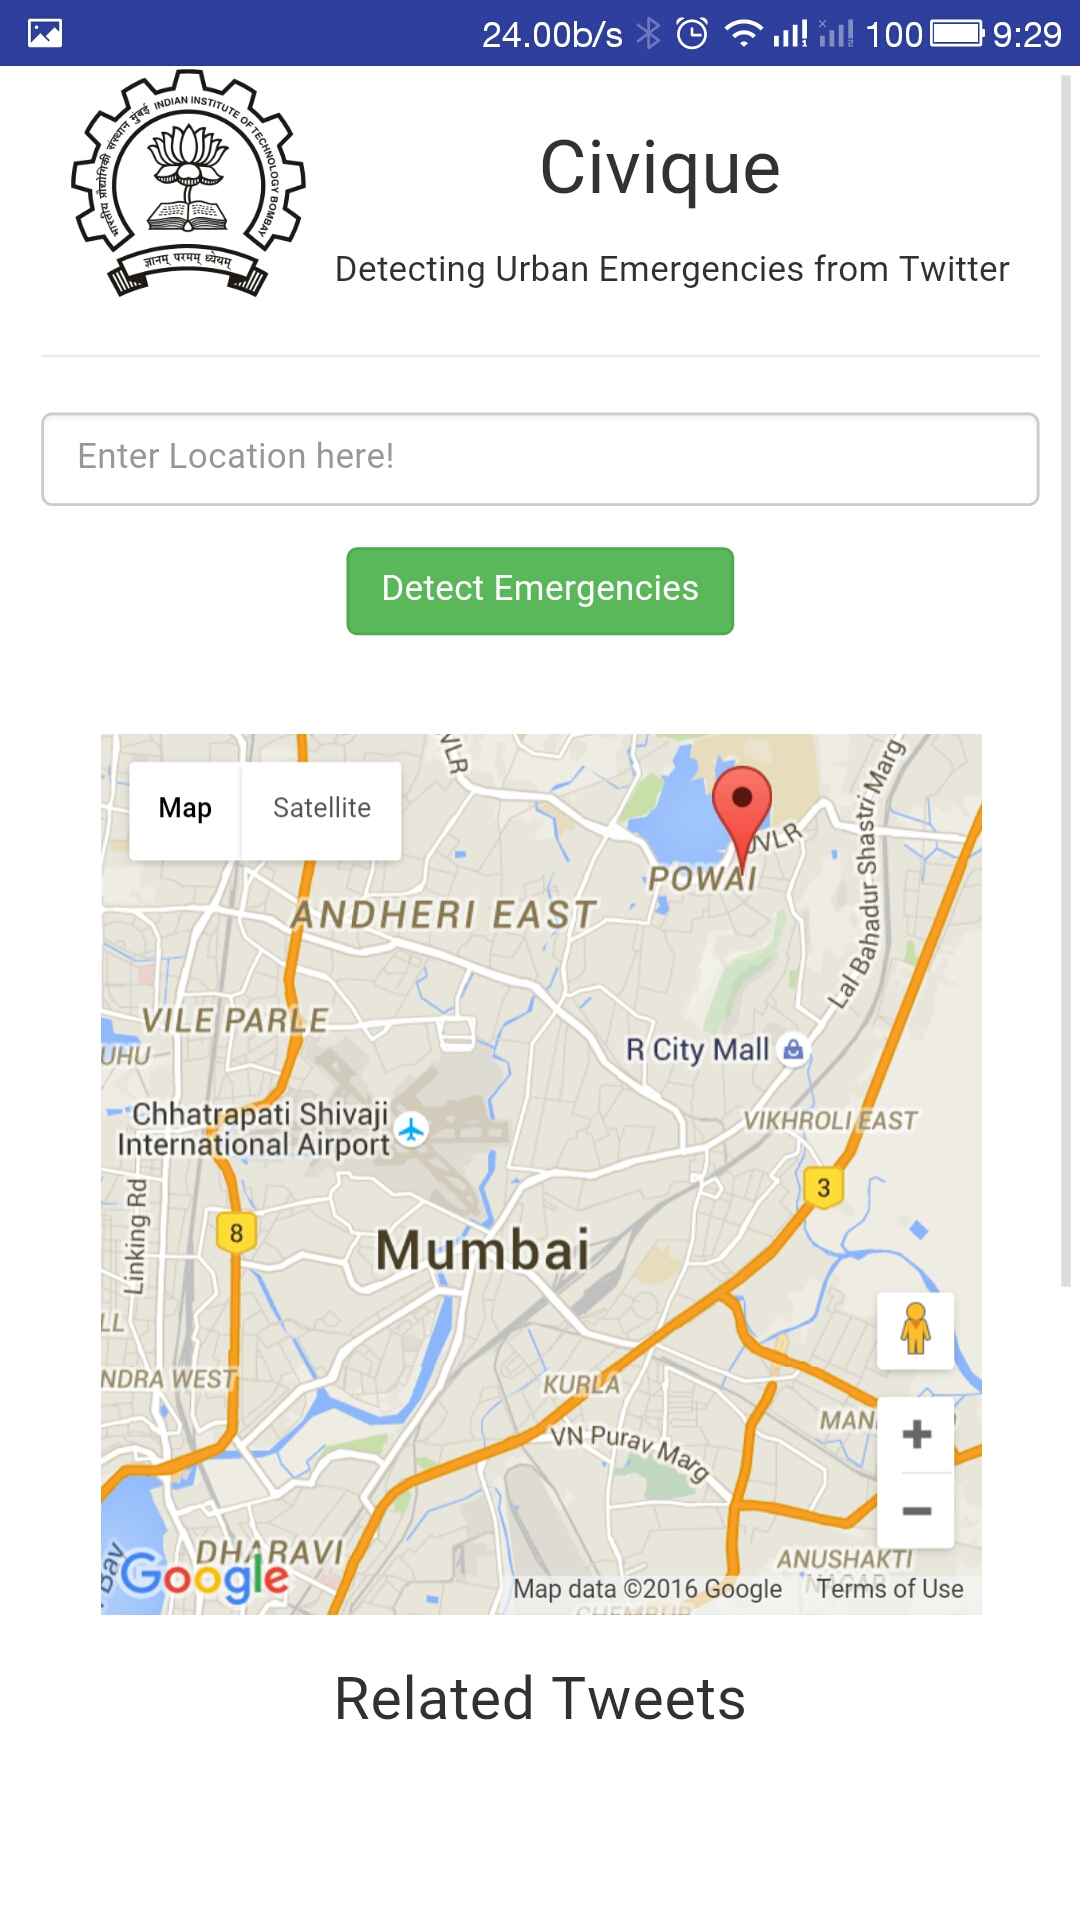
\includegraphics[height=10cm]{and1.jpg}}{\caption{Screenshot : Mobile interface}\label{fig:02}} \hspace{1cm}
\ffigbox[\FBwidth]
{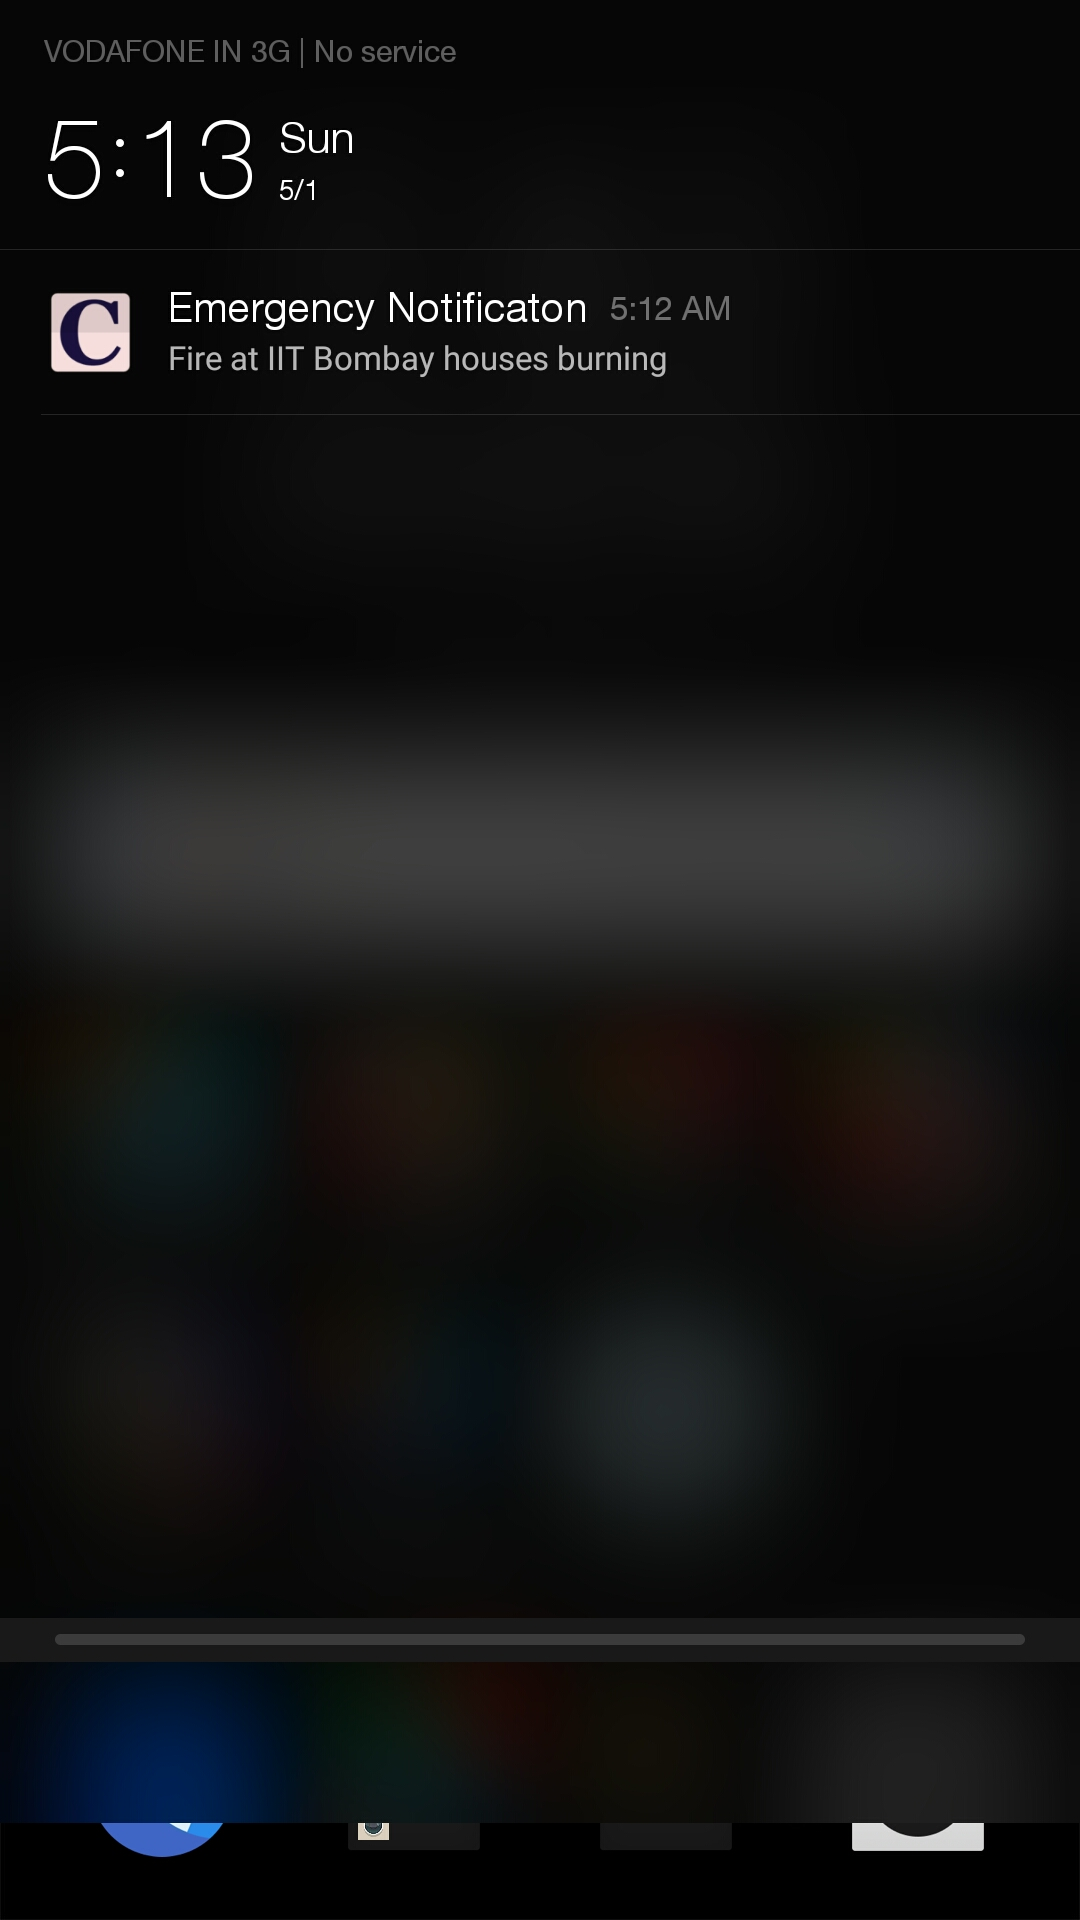
\includegraphics[height=10cm]{and2.jpg}}{\caption{Screenshot: Another Interface}\label{fig:03}}
\end{floatrow}}
\end{figure}
\vspace{-1cm}
The images have been put in, and they are side by side in the same
document on the same page. We have used the package floatrow and
graphicx to import images on Page 3. The images are from an Android
application I made for a project last semester. The table above are
values from an experiment we are doing in our lab. I am adding an
mathematical equation now just for the sake of it, because I think this is the only thing left to be demonstrated.\par
\begin{equation}
{NLL} = \sum_{i=1}^{N} \log{(P(s_{i}))} 
\end{equation}
where $s_{i}$  is the length of the $i^{th}$ saccade. \par
This text will refer to Equation 1 above. In case you would like to
see an alternative method to align the images, for instance images as subfigures, let me try to do it.\par
\newpage
\vspace*{0.5cm}
\begin{figure}
\centering
\begin{subfigure}{.5\textwidth}
  \centering
  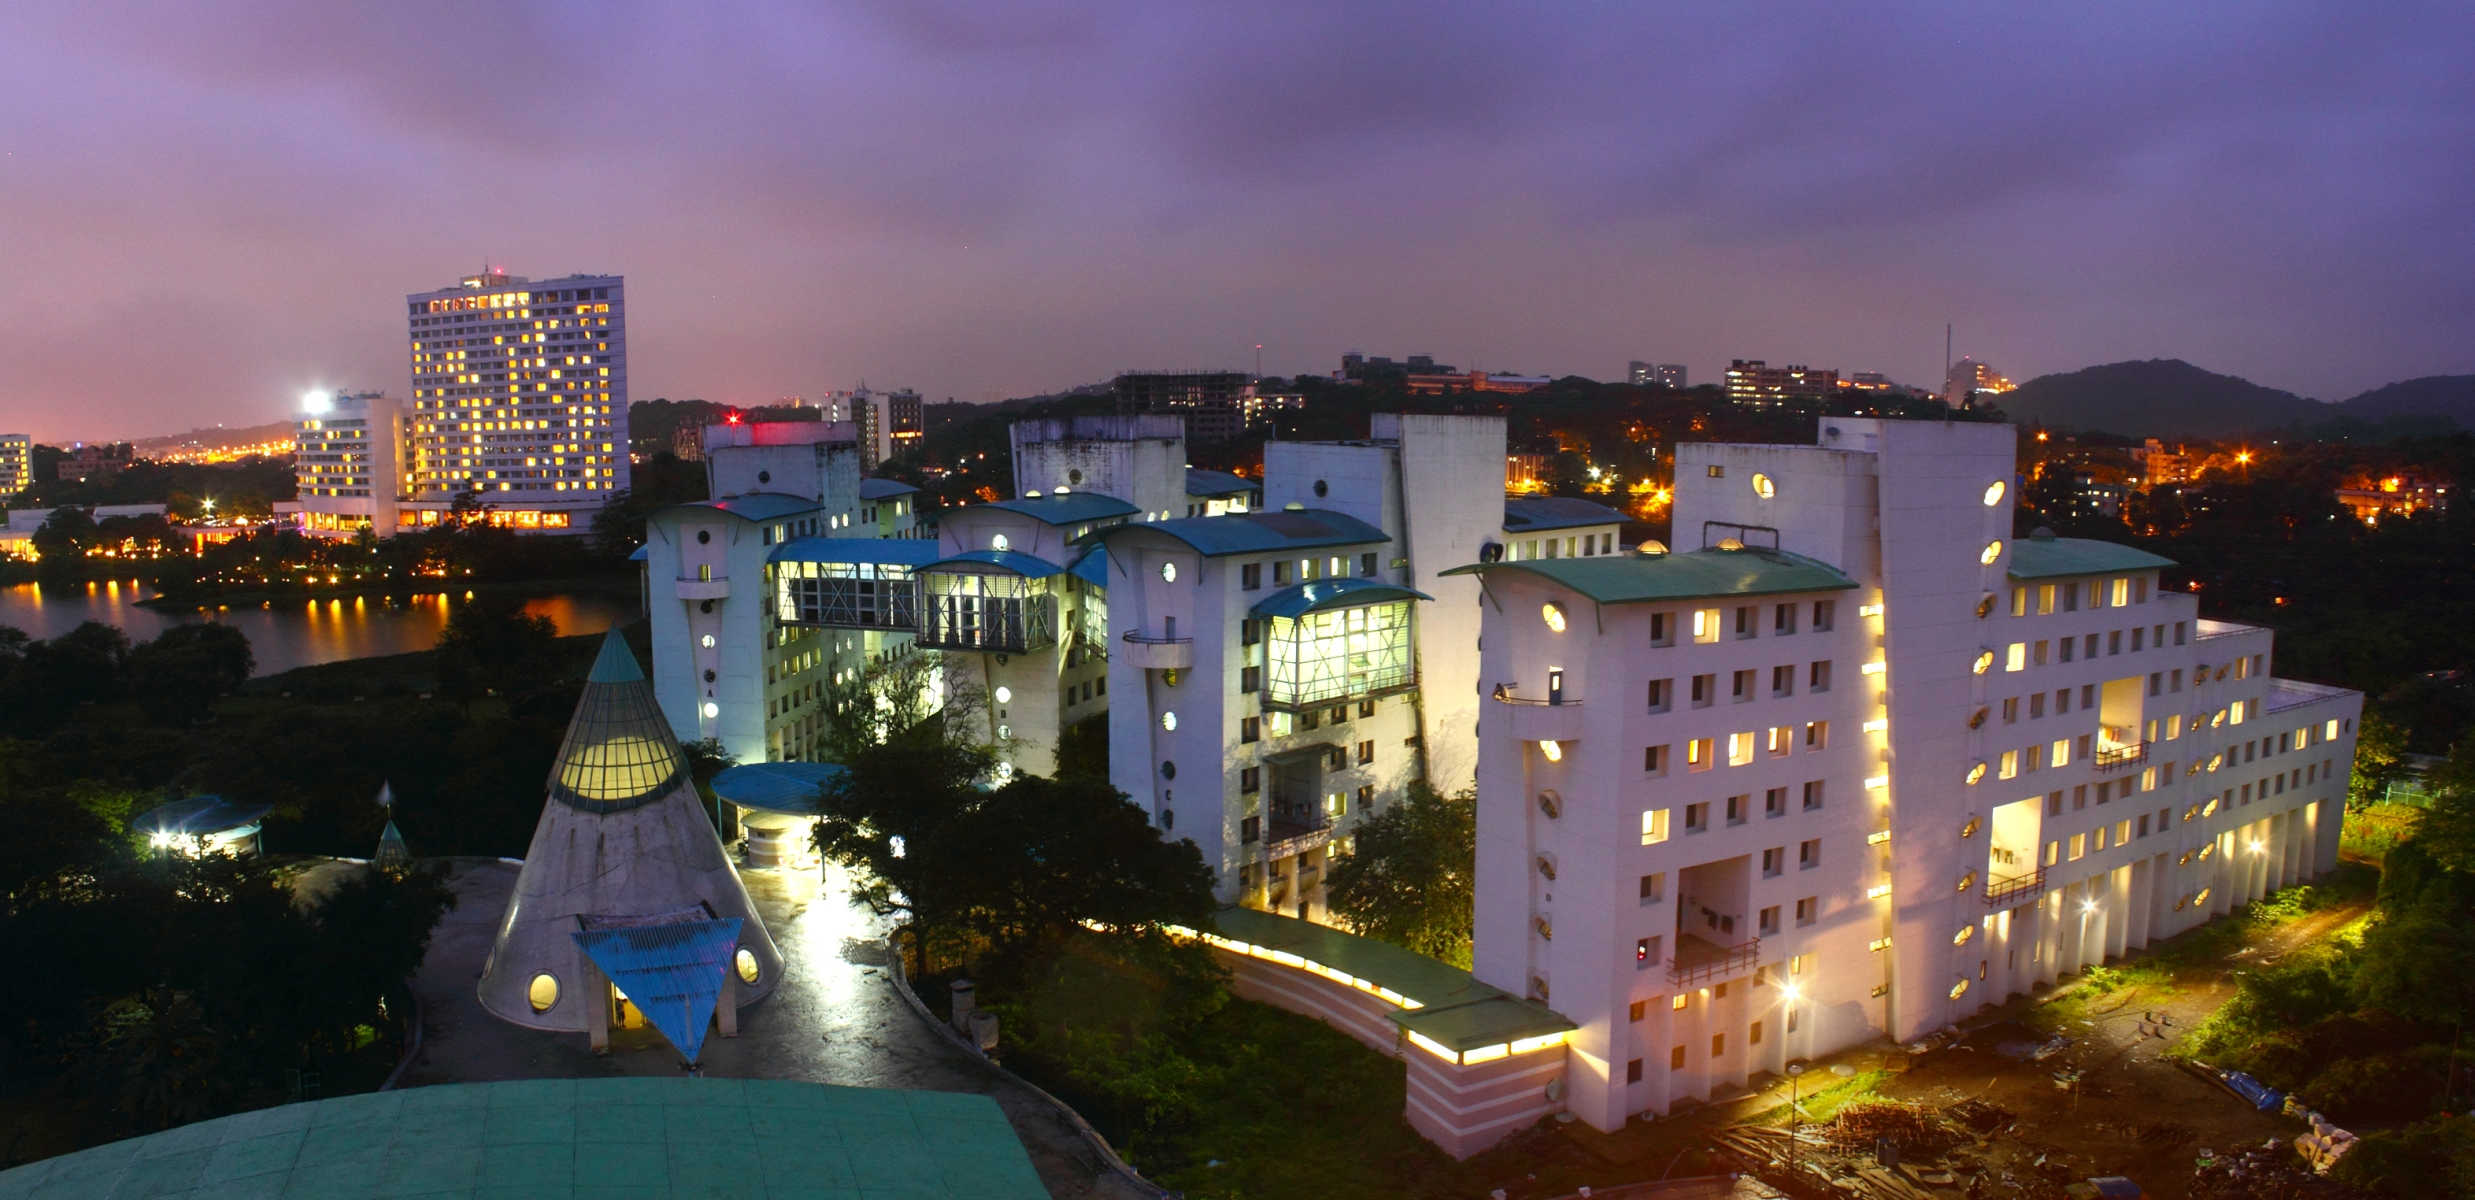
\includegraphics[height=3cm, width=.7\linewidth,]{img1.jpg}
  \caption{Caption 1}
  \label{fig:04}
\end{subfigure}% 
\hspace{-1.4cm}
\begin{subfigure}{.5\textwidth}
  \centering
  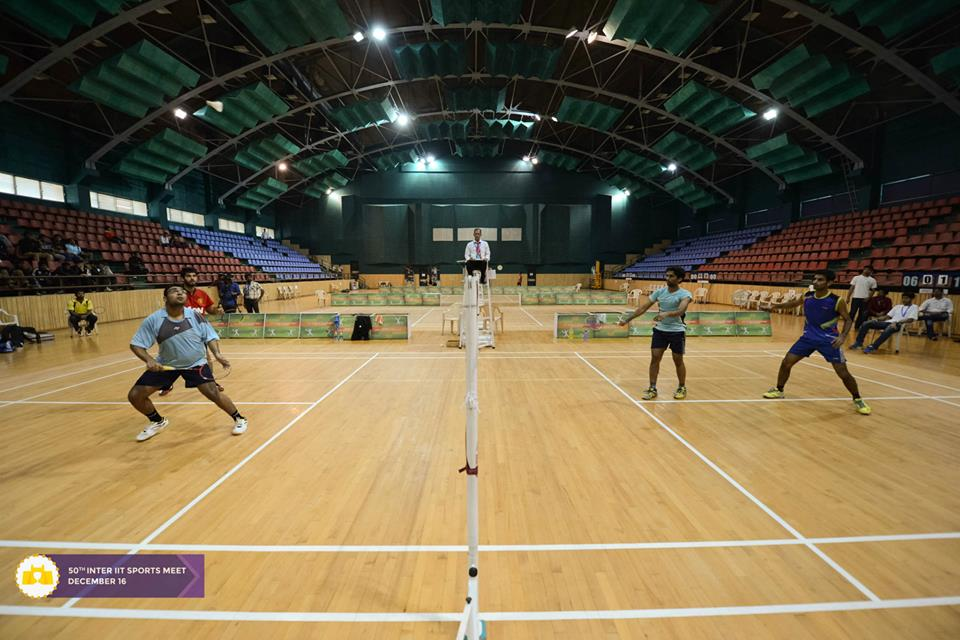
\includegraphics[height=3cm ,width=.7\linewidth,  ]{img2.jpg}
  \caption{Caption 2}
  \label{fig:05}
\end{subfigure}
\caption{Caption for this figure with two images}
\label{fig:test}
\end{figure}
\vspace{-1cm}
 This is another alternative to posting images in a \LaTeX Document, although you would still want me to put them in a table, since ‘The Document’ had them in a table. Let me try to do that.\\

\begin{table}[ht]
\caption{Table with images, finally !}
\begin{subfigure}{0.41\columnwidth}
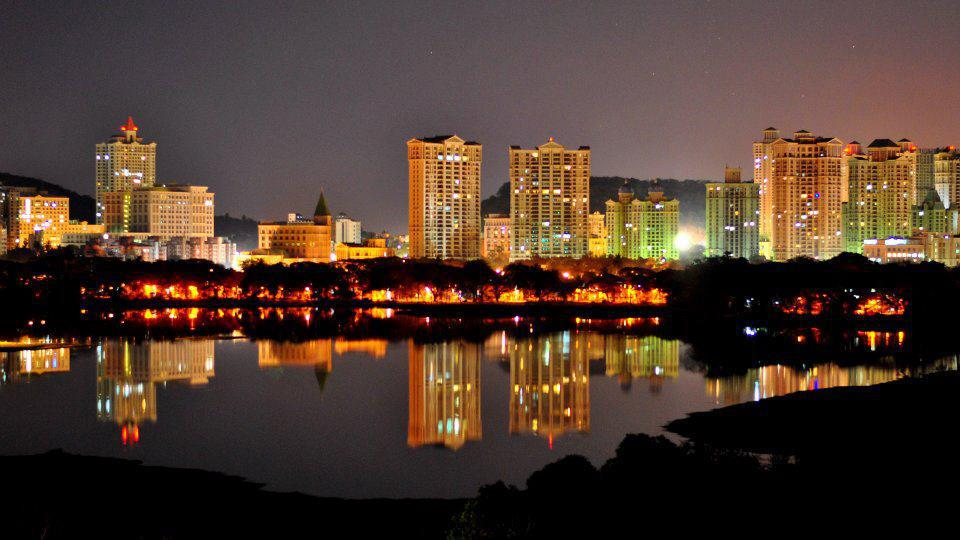
\includegraphics[width=1.3\linewidth]{img3.jpg}
    \label{fig:tablef1}
\end{subfigure}\hfill
\begin{subfigure}{0.41\columnwidth}
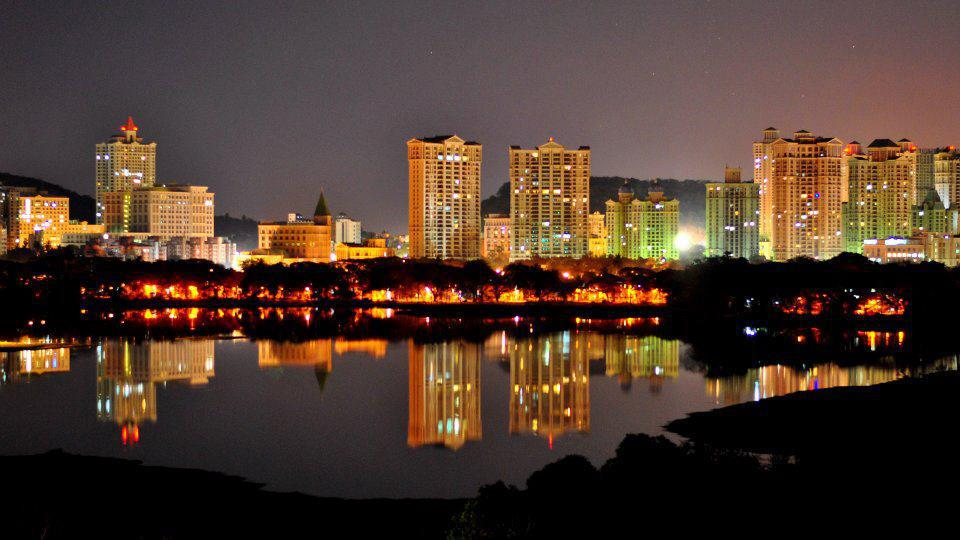
\includegraphics[width=1.3\linewidth]{img3.jpg}   
    \label{fig:tablef2}             
\end{subfigure}\\[1em]

\begin{subfigure}{0.41\columnwidth}
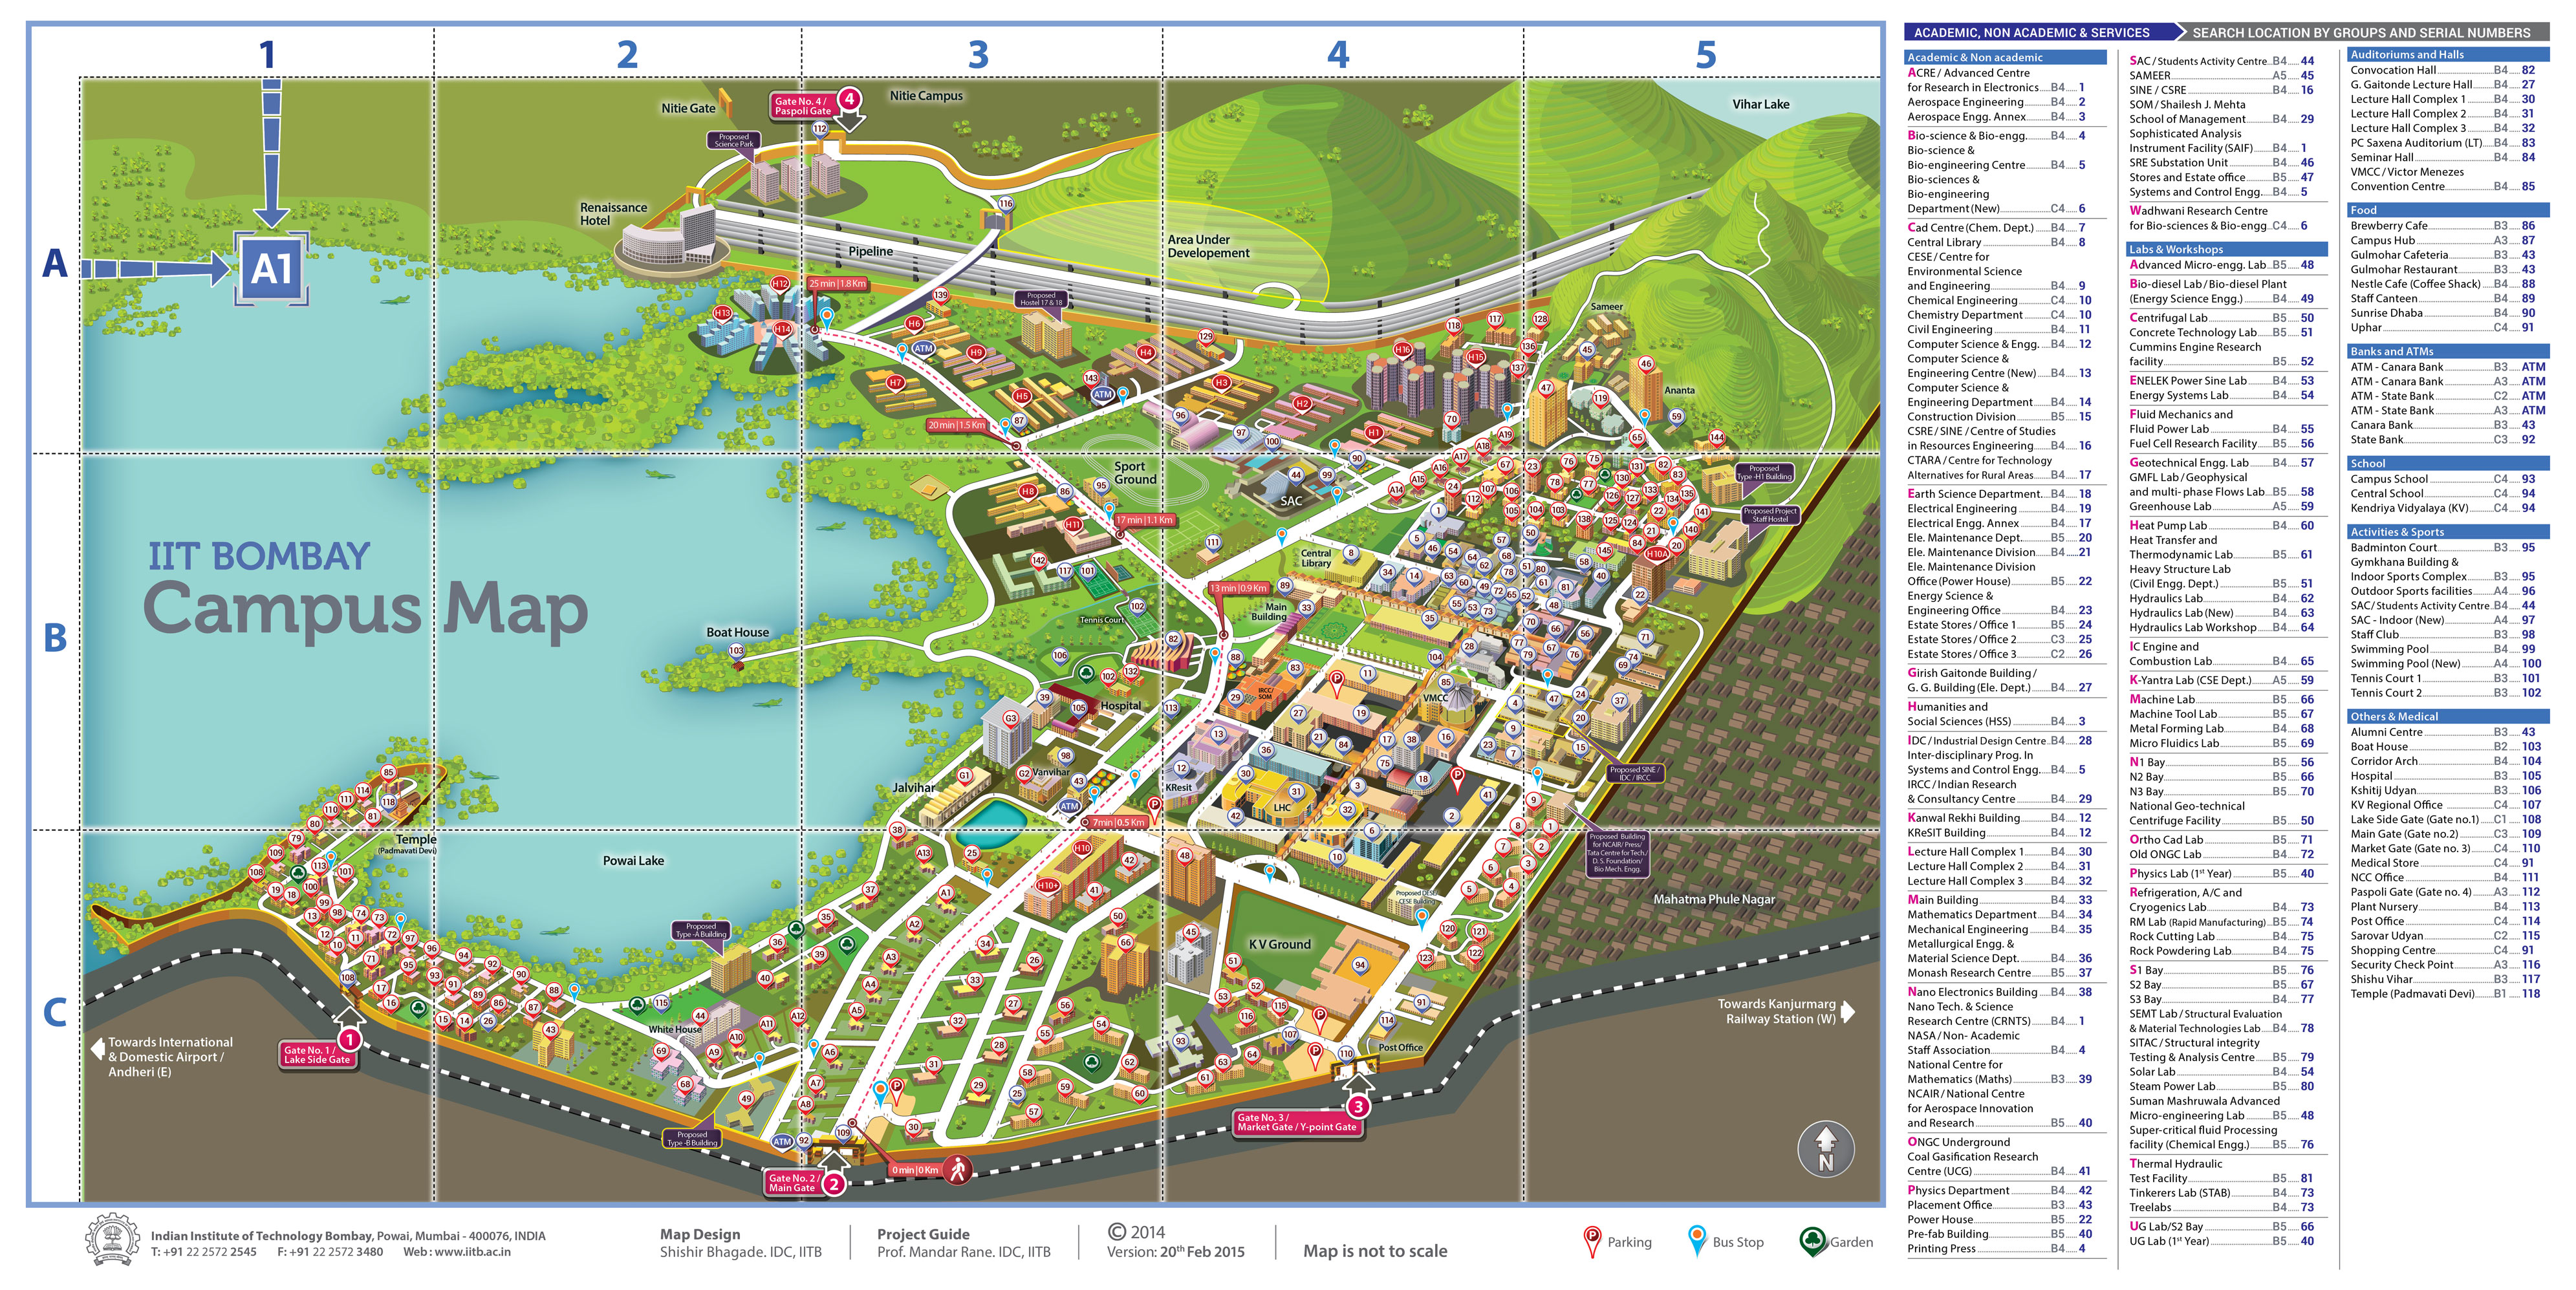
\includegraphics[width=1.3\linewidth]{img4.jpg}
    \label{fig:tablef3}
\end{subfigure}\hfill
\begin{subfigure}{0.41\columnwidth}
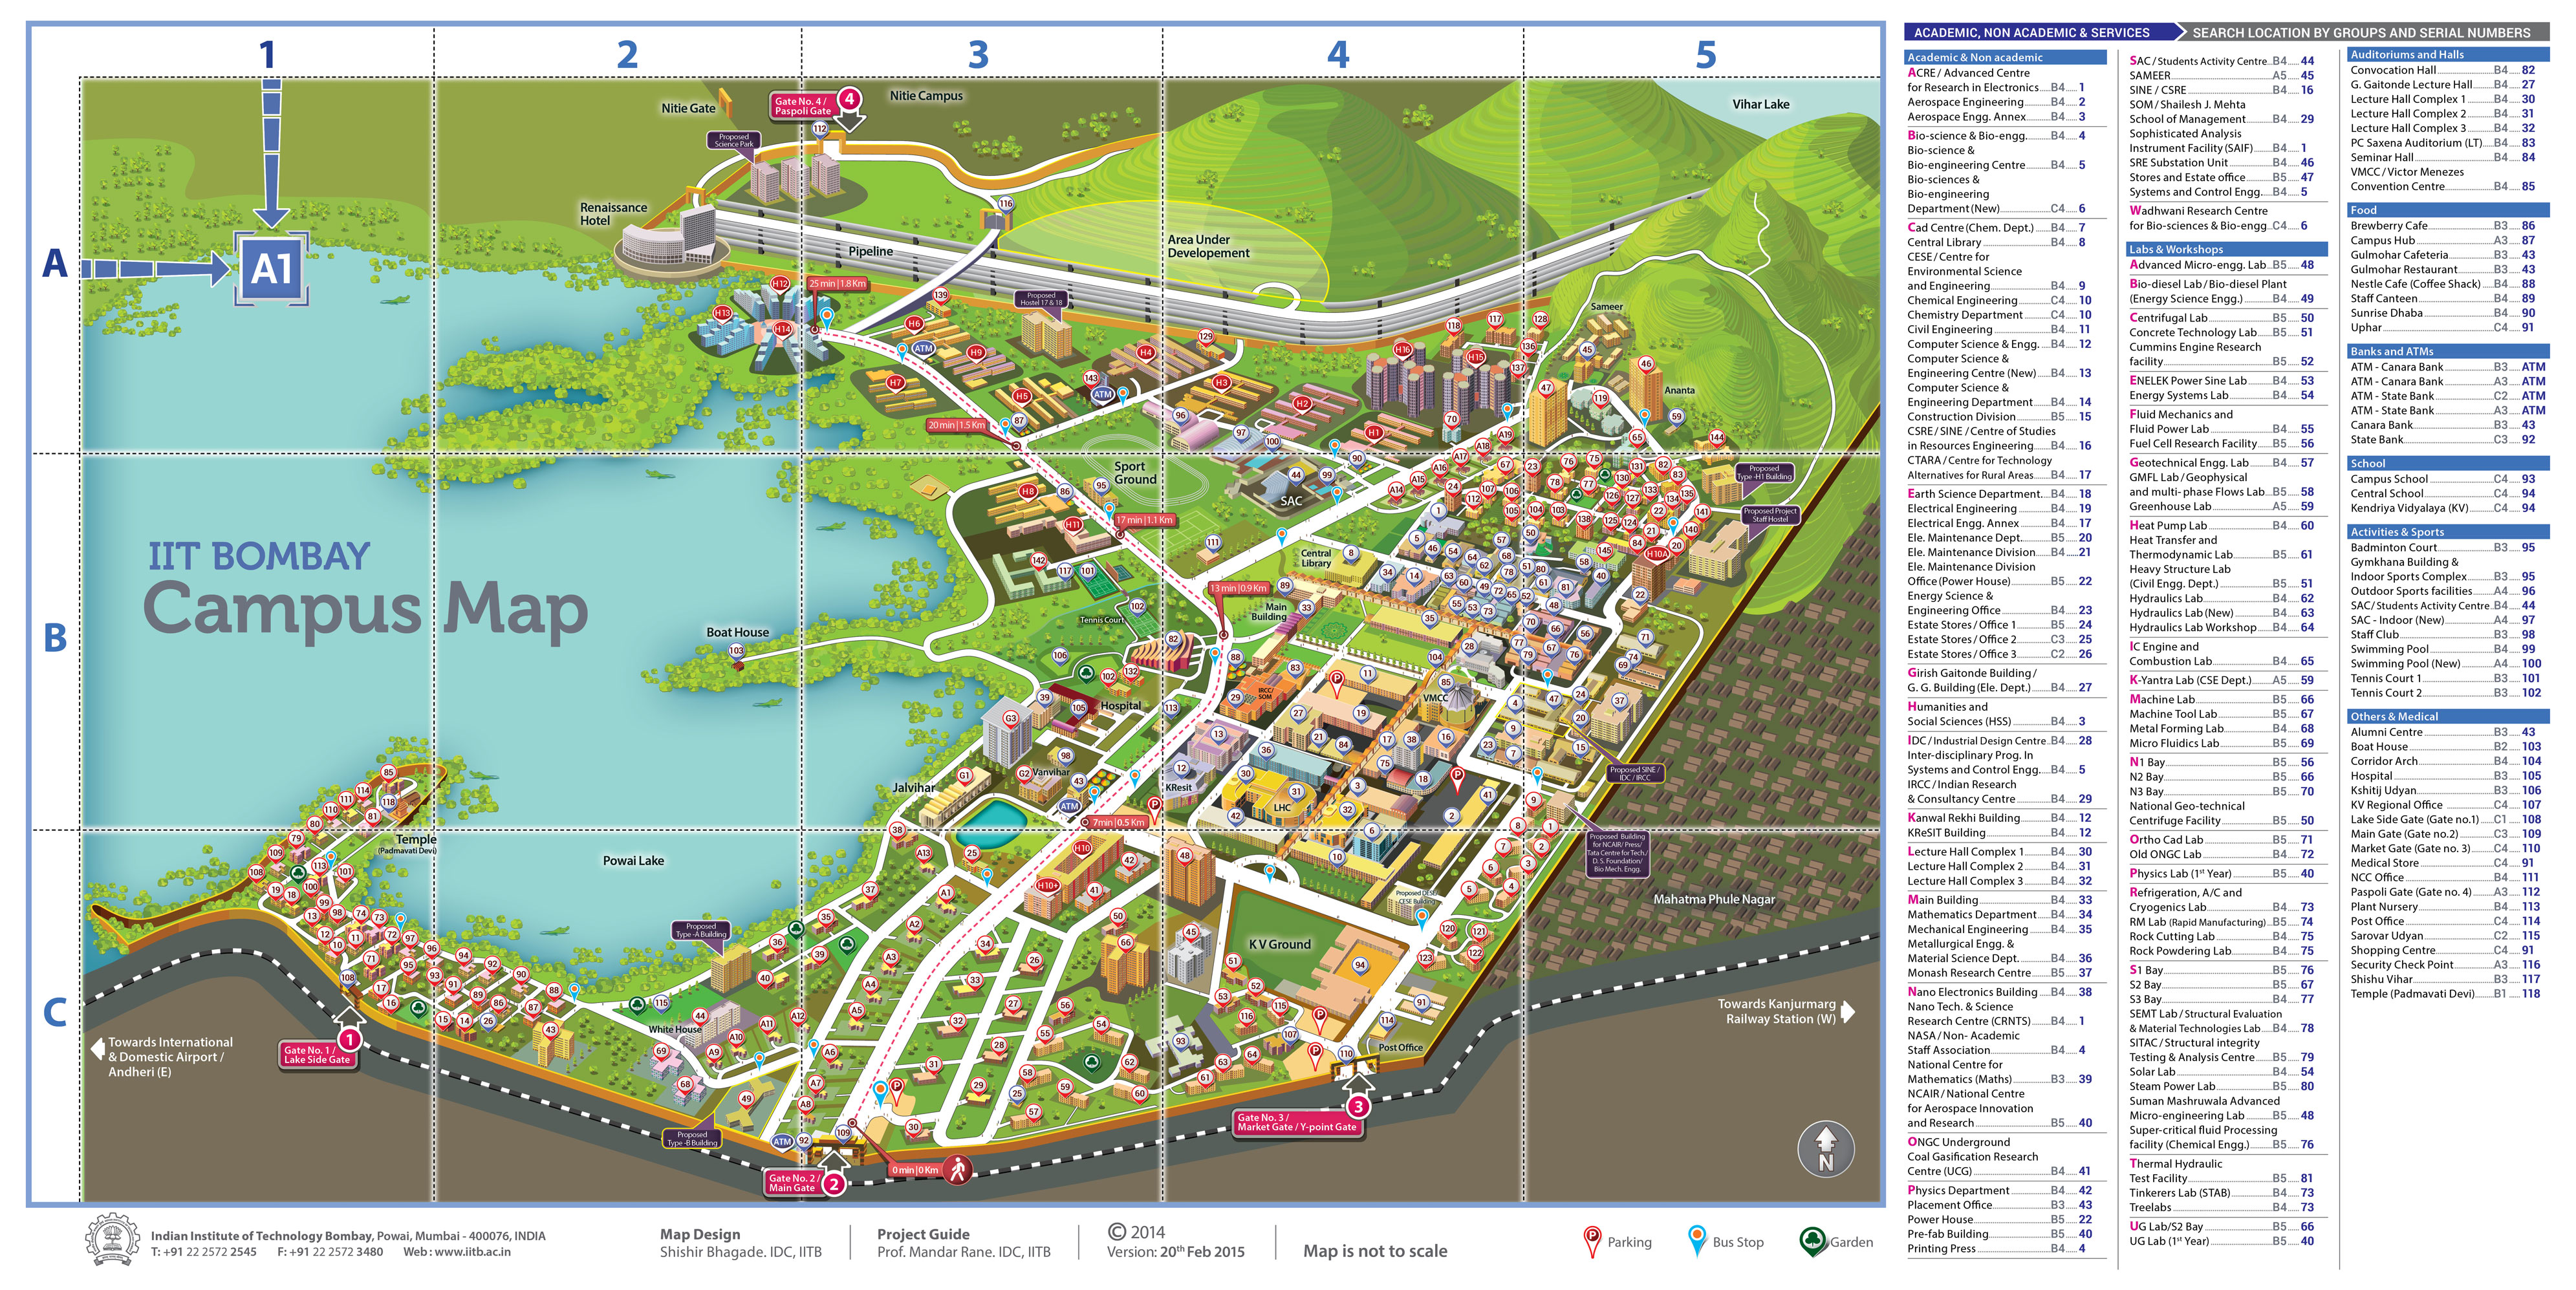
\includegraphics[width=1.3\linewidth]{img4.jpg} 
   \label{fig:tablef4}               
\end{subfigure}

\label{tab:mytable}
\end{table}
Now, that we have all the possible ways multiple images can be
aligned in the table. We will conclude this document with the final
section\par
\newpage
\vspace*{0.5cm}
{\noindent \Large \textbf{Conclusion}}\\

\noindent This document comprehensively demonstrated the capabilities of \LaTeX as
a document typesetting / desktop publishing package. \space We have used
various font size / family settings, we have used verbatim to display
Latex code in a latex document, image settings, sections, subsections,
references using labels, mathamatical equations, notations, use of ‘dia’
for creating a diagram / flowchart etc. \space I hope this suffices the need
of learning basic \LaTeX. I hope you also notice that the last section i.e.
Conclusion on Page 5 is unnumbered and displays the use of something.\\
  
\begin{thebibliography}{9}
\bibitem{latexcompanion} 
Pushpak Bhattacharyya.
Indowordnet.
\textit{In The WordNet in Indian
Languages}, pages 1--18. Springer, 2017.
\end{thebibliography} 

\end{document}
